\chapter{Systembeskrivelse}
Dette projekt omhandler som nævnt et Home Automation System, som kan anvendes til at simulere tilstedeværelse i et hjem, når ingen er hjemme. 
Dette sker ved at to lamper, et TV og en radio blandt andet tændes og slukkes på nogle foruddefinerede tidpunkter. 
Derved kan en indbrudstyv foranlediges til at tro, at nogen er hjemme, og derved kan indbrud forhindres. 

Systemet kan desuden anvendes til automatisering af brugerens hverdag, fx ved at bruge radio som vækkeur og tænde lys om morgenen, slukke alt lys om aftenen og lignende. 

Systemet er tilpasset én bestemt brugers hjem. 
Det er således ikke et universalt system, som umiddelbart kan tilpasses forskellige hjem med forskellige størrelser og behov. 
Systemet kan som nævnt styre to lamper, én radio og ét TV, herunder tænde, slukke og dimme lamper op og ned, samt anvende de mest almindelige funktioner for radio og TV (tænd, sluk, volumen, kanalvalg). 

\begin{figure} [h]
\centering
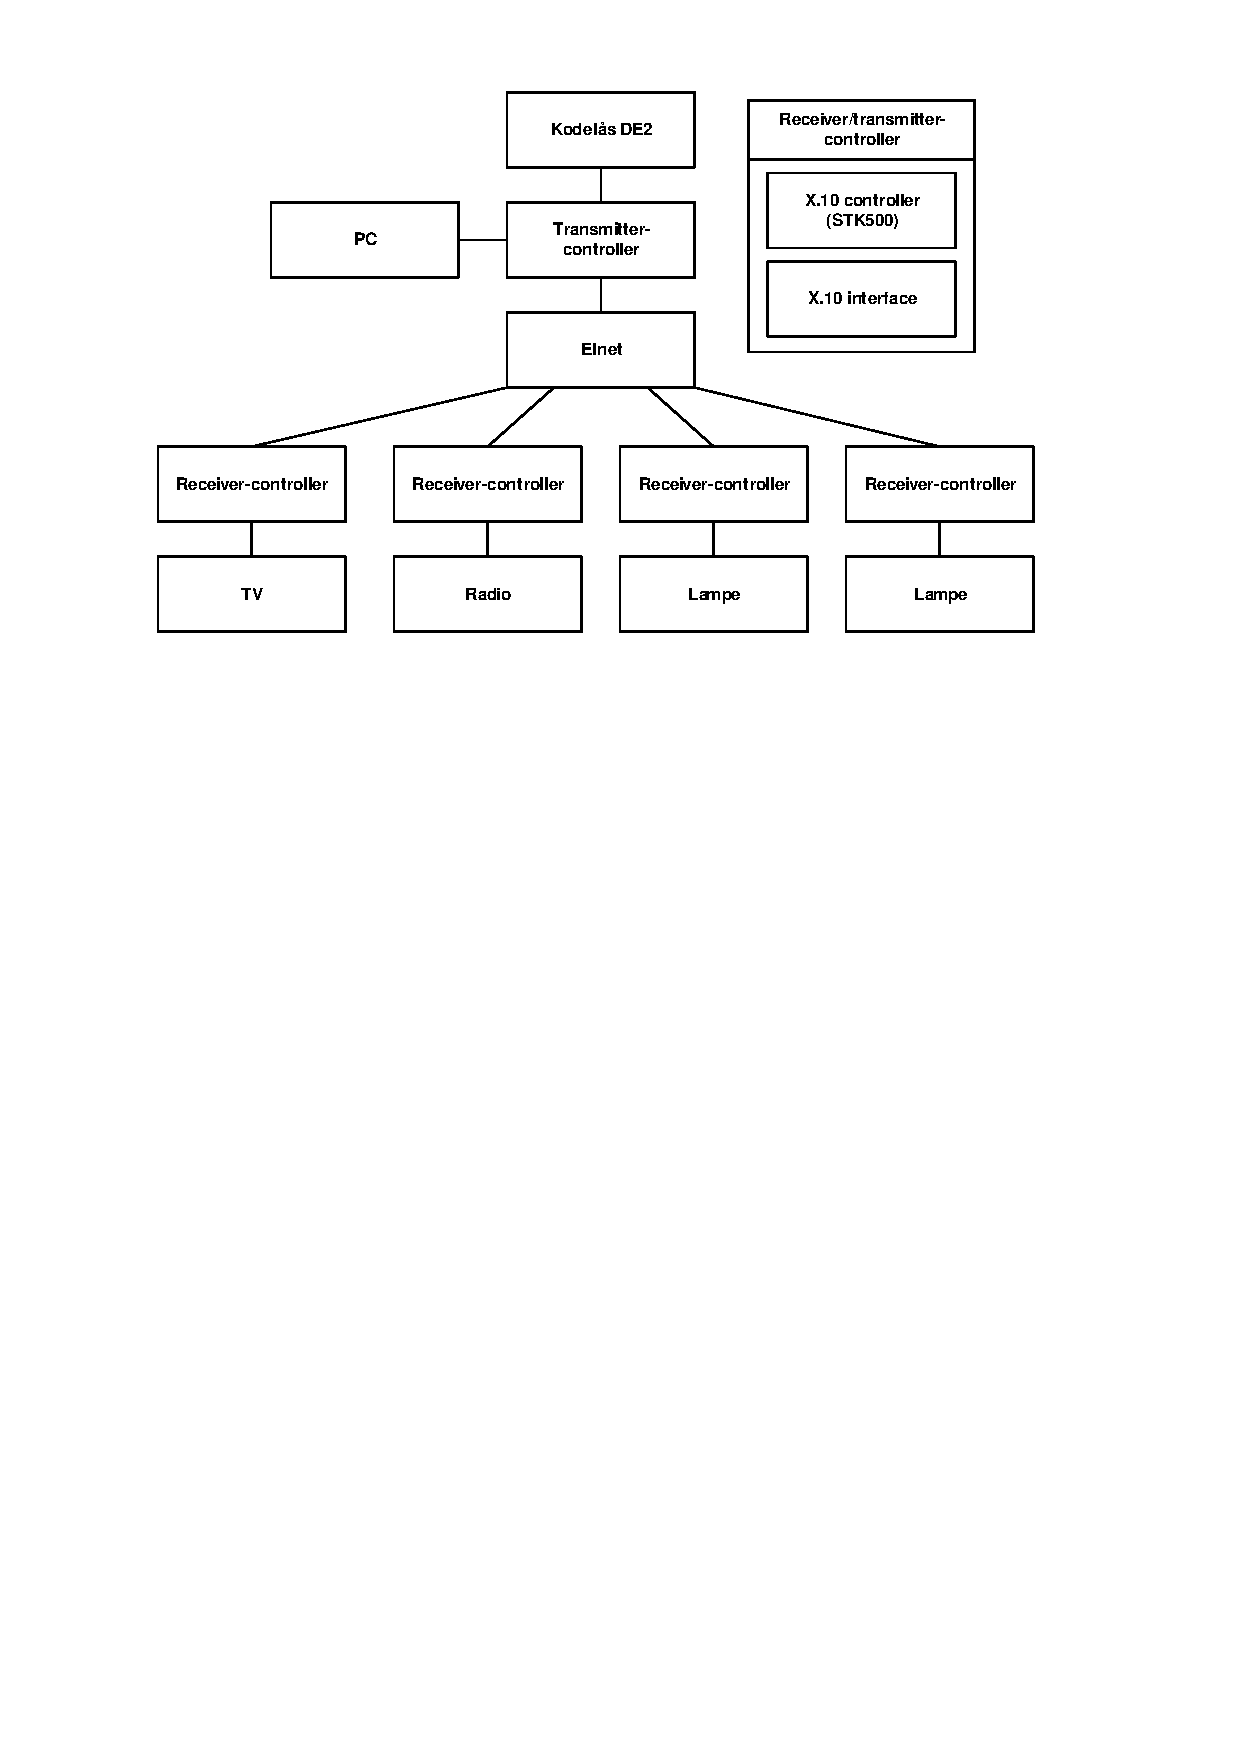
\includegraphics[scale=0.9,trim=50 535 80 40, clip=true] {../Projektdokumentation/Projektformulering/kommunikation_diagram.pdf}
\caption{Kommunikationsveje mellem enheder i systemet}
\end{figure}

Brugeren af systemet kan oprette et brugerdefineret scenarie, eller han kan vælge et af tre forudprogrammerede scenarier. 
Når et scenarie startes, simuleres tilstedeværelse i hjemmet ved at lamper, radio og TV tændes, slukkes etc. 
Et scenarie varer 24 timer og gentages indtil brugeren stopper det eller starter et andet scenarie. 
Et brugerdefineret scenarie gemmes ikke til senere brug, det eksisterer kun på transmitter controlleren så længe det afvikles. 

Der er i systembeskrivelsen lagt stor vægt på at systemet skulle være så simpelt som muligt. 
Dette er sket ud fra en tanke om at lille kompleksitet giver stor pålidelighed, samt at gruppen har valgt at fokusere på at lære så meget som muligt omkring processen i et ingeniørprojekt. 
Dette betyder selvfølgelig også en begrænset funktionalitet, men det er forsøgt at finde et fornuftigt leje, som sikrer udfyldelse af systemets mål. 
Der er således rimelig begrænset funktionalitet i systemets software, fx gemmes brugerdefinerede scenarier ikke. Hardwaren er opdelt i underdele – byggesten – hvoraf nogle genanvendes flere steder i systemet. 
Systemet indeholder kun envejskommunikation, dvs. den centrale transmitter modtager ikke informationer om en afsendt kommandos gennemførelse, hvilket kunne have givet ekstra sikkerhed for funktionaliteten. 

For yderligere information henvises til \textit{systembeskrivelsen} på side \pageref{P-Systembeskrivelse} i dokumentationen. 

\clearpage